\subsection{Considered Data Centre Architectures}\label{sec:cloud:data_centers:problem_formulation}

A widely used data centre architecture is the three-tier architecture shown in \reffig{fig:cloud:data_centers:problem_formulation:3-tier_datacenter}.
The upper two layers of the architecture are responsible for distributing the traffic and consist of layer 3 switches where each switch has a backup switch.
In this section, we focus on the edge layer and especially on a single \gls{POD}.
A \gls{POD} consists of a number of servers connected over top of rack switches to an aggregation switch.

\begin{figure}
  \centering
  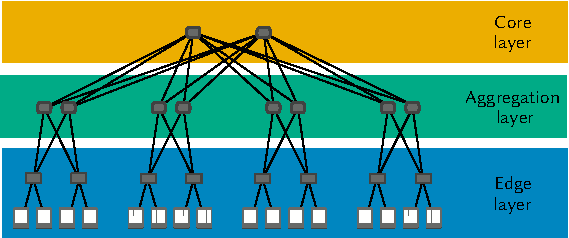
\includegraphics{cloud/data_centers/problem_formulation/figures/architecture}
  \caption{Considered standard three-tier data centre architecture.}
  \label{fig:cloud:data_centers:problem_formulation:3-tier_datacenter}
\end{figure}

We assume that new jobs entering the system arrive with exponentially distributed inter-arrival time.
When a job arrives at the \gls{POD}, it is forwarded to an idle server.
If no idle server is available, the job is queued.
Once a server finishes processing its current job, it picks another one from the queue.

Our goal is to evaluate how much power is consumed in a data centre and how much can be saved when servers, currently not processing any job, are switched off.
Therefore, we developed two different data centre models.
The first model, the \emph{traditional data centre}, consists of two-state servers only which are either \emph{busy} or \emph{idle}, as shown in \reffig{fig:cloud:data_centers:problem_formulation:servers:idle_busy} 
For the second model, a more \emph{energy-efficient data centre}, a subset of the servers may additionally be switched \emph{on} and \emph{off} on demand, shown in \reffig{fig:cloud:data_centers:problem_formulation:idle_busy_off} as recommended in~\cite{EPA2007}.

\begin{figure}
	\begin{subfigure}[b]{\textwidth}
	\centering
	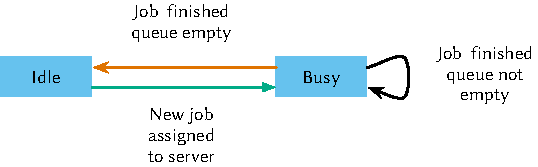
\includegraphics{cloud/data_centers/problem_formulation/figures/idle_busy}
	\caption{2-state server model}\label{fig:cloud:data_centers:problem_formulation:servers:idle_busy}
	\end{subfigure} 
	\begin{subfigure}[b]{\textwidth}
	\centering
	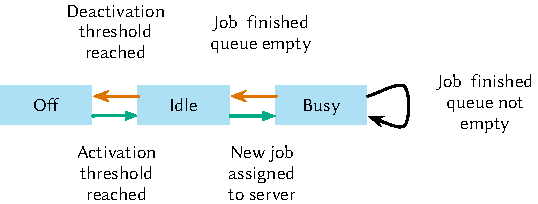
\includegraphics{cloud/data_centers/problem_formulation/figures/idle_busy_off}
	\caption{3-state model of a reserved server}\label{fig:cloud:data_centers:problem_formulation:idle_busy_off}
	\end{subfigure}

	\caption{Assumed power state transition on a per server level.}\label{fig:cloud:data_centers:problem_formulation:servers}
\end{figure}

\subsubsection*{Traditional Data Centre}\label{sec:cloud:data_centers:problem_formulation:default_data_center}
For the traditional data centre model, each of the \(n\) servers is either on and processing a job or on and idle as depicted in \reffig{fig:cloud:data_centers:problem_formulation:servers:idle_busy}.
If a busy server finishes processing a job and the queue is empty, the server becomes idle. Once a new job is assigned to a yet idle server, the server becomes busy.
According to our measurements of a server with an Intel twelve core processor \SI{2.67}{\giga\hertz} and \SI{32}{\giga\byte} RAM, a server currently processing a job consumes \(e_{\text{busy}} = \SI{240}{\watt}\).
An idle server still consumes \(e_{\text{idle}} = \SI{170}{\watt}\).

\subsubsection*{Energy-Efficient Data Centre}\label{sec:cloud:data_centers:problem_formulation:energy_efficient_data_center}
For the second model, we differentiate between two types of servers:
\(n\) base-line servers which are always on and \(m\) reserved servers to be enabled on demand.
If they are enabled, their power drain is similar to that of the default data centre model.
If they are disabled, each server consumes \(e_\text{off} = \SI{0}{\watt}\).
The \(n\) servers which are always enabled consume the same power as in the default data centre model.
If the system queue has a length exceeding \(\theta_2\) where \(\theta_2 \in (0, m)\) holds, the \(m\) reserved servers are enabled and stay enabled until the total number of jobs in the system drops to \(\theta_1\) for \(\theta_1 \in (0, n)\).
The transition between power levels for each of the reserved servers is depicted in \reffig{fig:cloud:data_centers:problem_formulation:idle_busy_off}.

The energy-efficient data centre operation model with the parameters \(\theta_1\) and \(\theta_2\) is depicted in \reffig{fig:cloud:data_centers:problem_formulation:model} and described in detail in the next section.

\begin{figure}
  \centering
  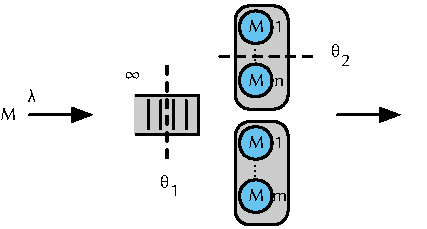
\includegraphics{cloud/data_centers/problem_formulation/figures/model}
  \caption{Considered system model for an energy-efficient data centre.}
  \label{fig:cloud:data_centers:problem_formulation:model}
\end{figure}